\section{B-Tree}

\subsection{Optimal $b$}

Since we know that B-Trees play well with memory hierarchy, we want to be able to perfectly fit a node into a cache block for fast access.
In general, $b$ should be based on the size of the key-value pair when stored in memory especially if they could have a variety of sizes.
However, consider the case where both the key and the value are pointers or a reference type (similar to in Java).
The amount of memory required for one key-value pair would be 128 bits or 16 bytes on a modern 64-bit machine.

Assume that the B-Tree is storing a pair of pointers for key and value and recall that a modern computer's cache line size is typically 64 bytes. This means that we would be able to perfectly fit 4 pairs of keys and values into a single cache line for fastest access. Therefore, the optimal value for $b$ would be 4 based on the these assumptions. Note that this $b$ would go up as the size of the key-value pair goes down, but $b = 4$ should be a good baseline.

\subsection{B-Tree vs. Ordered Map}

On the testing machine, the best performance comes from when $b = 18$. However, the performance is still very lacking compared to a built-in ordered map in C++ as the B-tree (with poor implementation) is approximately around \textit{7-12 times slower than the built-in ordered map}. Maybe I just write bad code. Below are the results from the experiments.

\subsubsection{Results}

\subsubsection*{Insertion}

\begin{figure}[H]
	\begin{center}
		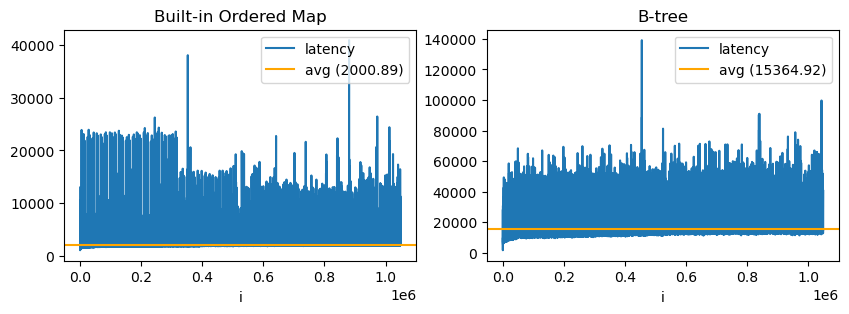
\includegraphics[width=0.9\textwidth]{05-insert-latencies.png}
		\caption{Insert latency of a C++ built-in ordered map and a B-tree}
		\label{fig:05-insert-latency}
	\end{center}
\end{figure}

\subsubsection*{Search}

\begin{figure}[H]
	\begin{center}
		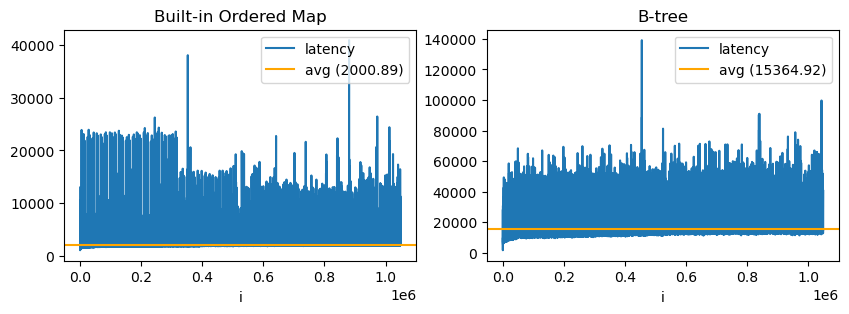
\includegraphics[width=0.9\textwidth]{05-insert-latencies.png}
		\caption{Search latency of a C++ built-in ordered map and a B-tree}
		\label{fig:05-search-latency}
	\end{center}
\end{figure}
